\subsection{Login}
This subsystem is a graphical user interface that allows a user to log into Synthify

\begin{figure}[h!]
	\centering
 	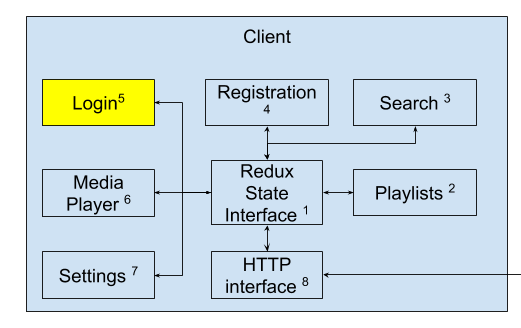
\includegraphics[width=0.60\textwidth]{images/client/client_login.png}
 	\caption{Login subsystem}
\end{figure}

\subsubsection{Assumptions}
One assumptions made is that the user will have an account in order to login.

\subsubsection{Responsibilities}
The login page will be responsible for recording the user's email and password, which will be sent to the Server subsystem via the HTTP interface.

\subsubsection{Subsystem Interfaces}
\begin {table}[H]
\caption {Login interfaces} 
\begin{center}
    \begin{tabular}{ | p{1cm} | p{6cm} | p{3cm} | p{3cm} |}
    \hline
    ID & Description & Inputs & Outputs \\ \hline
    \#xx & User found & \pbox{3cm}{User's E-mail \\ User's Password} & \pbox{3cm}{HTTP 200 OK, JSON object containing information}  \\ \hline
    \#xx & User not found or password incorrect & \pbox{4cm}{Invalid Login E-Mail \\ Incorrect Password} & \pbox{3cm}{HTTP 404, JSON Object containing error message}  \\ \hline
    \end{tabular}
\end{center}
\end{table}

\newpage
